

\chapter{Estudo de Caso e Metodologia}

Neste capítulo é apresentado o estudo de caso, onde os dados públicos do programa Bolsa Família são inseridos e extraídos de um banco de dados não relacional Cassandra, com \emph{clusters} de um, dois, quatro e seis máquinas, além das descrições das etapas e programas utilizados. O programa é exposto brevemente e o modelo de dados e o ambiente utilizado são descritos.

\section{Estudo de Caso}
O Bolsa Família é um programa federal, em operação desde 2003 quando foi instituído pelo então presidente Lula, com objetivo de "combater a fome e promover a segurança alimentar e nutricional, combater a pobreza e outras formas de privação das famílias e promover o acesso à rede de serviços públicos, em especial, saúde, educação, segurança alimentar e assistência social"~\cite{caixa-bolsafamilia}. 
O programa se caracteriza pela transferência de renda para famílias brasileiras em situação de pobreza e extrema pobreza, ou seja, que recebam até R\$170 e R\$85 respectivamente. Atualmente cerca de 13,9 milhões de famílias são atendidas pelo programa, recebendo em média R\$182 cada, totalizando R\$27,4 bilhões em 2016, que recebem recursos do Ministério do Desenvolvimento Social, por meio da Caixa Econômica Federal~\cite{gov-bolsafamilia1, gov-bolsafamilia2}.

Os dados do Bolsa Família utilizados para estudo de caso nesse trabalho foram obtidos no \emph{site} do Portal da Transparência, um projeto da Controladoria Geral da União, que disponibiliza informações sobre os gastos do dinheiro público, com objetivo de melhora na transparência da gestão pública~\cite{sobreportaldatransparencia}. 

Esses dados são disponibilizados em formato aberto \emph{.csv}, e agrupados mensalmente, trazendo informações sobre a transferência de recursos federais aos participantes do programa. 

Foram utilizados no total vinte quatro arquivos, equivalentes a vinte e quatro meses do programa, compreendidos entre Julho de 2014 e Junho de 2016. Cada arquivo possui em média 16GiB de tamanho e 13.968.749 registros.

Cada arquivo apresenta como campos: \textbf{UF, Código SIAFI Município, Nome Município, Código Função, Código Subfunção, Código Programa, Código Ação, NIS Favorecido, Nome Favorecido, Fonte-Finalidade, Valor Parcela e Mês Competência}. Um subconjunto dessas colunas foi escolhido para a realização dos testes, como será explicado na próxima sessão.

No trabalho os dados foram inseridos em um ambiente de \emph{cluster} de até seis máquinas, com configuração de \emph{hardware} com Intel i5-4570 3.20GHz, 16GB de RAM, disco rígido de 500GB, com sistema operacional Ubuntu.

\section{Modelo de dados Cassandra}
O modelo de dados do Cassandra foi criado utilizando-se um \emph{keyspace} com fator de replicação de apenas um~\ref{lst:cql_create_keyspace}, pois a tolerância a falhas não é um fator relevante nos testes a serem realizados, devido ao ambiente controlado em que eles são feitos.

O Cassandra apresenta duas estratégias de replicações de dados, a \emph{SimpleStrategy} e a \emph{NetworkTopologyStrategy}, sendo a primeira utilizada em \emph{datacenters} únicos e com apenas um \emph{rack}, e a segunda para uso em múltiplos \emph{datacenters}. Devido ao ambiente restrito do laboratório utilizado, foi escolhida a \emph{SimpleStrategy} como estratégia de replicação dos dados.

\noindent
\begin{minipage}[c]{1\textwidth}
\begin{lstlisting}[caption={Código CQL criação do keyspace},label={lst:cql_create_keyspace},language=SQL]
CREATE KEYSPACE bolsa_familia WITH replication = {'class': 'SimpleStrategy', 'replication_factor': 1};
\end{lstlisting}
\end{minipage}

Apenas uma família de colunas foi criada, contendo as colunas \textbf{UF, Código SIAFI Município, Nome Município, NIS Favorecido, Nome Favorecido, Fonte-Finalidade, Valor Parcela, Mês Competência}. Esse subconjunto foi escolhido pois os testes não buscam uma análise e interpretação das informações armazenadas, e sim mensurar o desempenho de um banco de dados distribuídos com dados públicos abertos.

Ao se definir uma chave primária no Cassandra é necessária a escolha de uma \emph{Partition Key} (chave de partição) e uma \emph{Clustering Key} (chave de agrupamento). A \emph{Partition Key} é responsável pela distribuição dos dados nos nós do ambiente, enquanto a \emph{Clustering Key} distribui esses dados dentro de cada nó.

Para o modelo testado foi escolhido como \emph{Partition Key} apenas a coluna \textbf{UF} como forma de distribuição dos registros no \emph{cluster}. Além disso, para complementar a chave primária foram escolhidos os campos \textbf{NIS Favorecido, Valor Parcela e Mês Competência}, que identificam unicamente cada registro, considerando que um mesmo favorecido pelo programa(identificado pela coluna NIS Favorecido), pode receber mais de uma parcela em um mesmo mês, ou parcelas em meses distintos. A figura \ref{fig:modelocassandra} apresenta o modelo utilizado.

\begin{figure}[!htb]
	\centering
	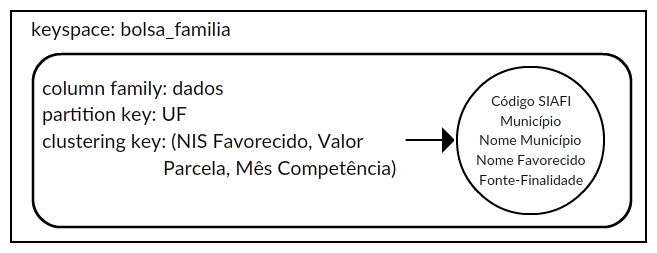
\includegraphics[width=1\textwidth]{figuras/modelocassandra.png}
	\caption{Modelo de Dados}
	\label{fig:modelocassandra}
\end{figure}

Foi feito também um ordenamento das colunas, definindo Período e NIS Favorecido em ordem crescente e valor em ordem decrescente~\ref{lst:cql_create}. 

\begin{lstlisting}[caption={Código CQL criação da tabela},label={lst:cql_create},language=SQL]
CREATE TABLE bolsa_familia.dados (uf text, periodo timestamp, valor double, nis_favorecido bigint, cod_municipio int, fonte text, nome_favorecido text, nome_municipio text, PRIMARY KEY(uf, periodo, valor, nis_favorecido)) WITH CLUSTERING ORDER BY(periodo ASC, valor DESC, nis_favorecido ASC);
\end{lstlisting}

A configuração do ambiente Cassandra foi feita por meio do cliente \emph{cqlsh}, que permite a realização de consultas e manipulações no banco por meio da linguagem \emph{CQL}(\emph{Cassandra Query Language}).

\section{Linguagem CQL}
A linguagem \emph{CQL}(\emph{Cassandra Query Language}), introduzida na versão 0.8 do Cassandra~\cite{cassandra08} é uma linguagem de \emph{script}, utilizada como interface padrão para um banco de dados Cassandra, sendo então a maneira recomendada de interação com o mesmo~\cite{cassandracql}. 

Sua utilização é similar à do SQL convencional, com a abstração de tabelas sendo constituídas por colunas e linhas. Devido à natureza desnormatizada do um modelo de dados em um banco Cassandra, o CQL possui limitações no uso de queries consideradas mais complexas, como joins e subqueries~\cite{cassandracql}.

Para interação direta com o banco também é disponibilizado o \emph{cqlsh}(\emph{CQL shell}), um utilitário desenvolvido em Python, que por meio de linha de comando permite a execução de chamadas CQL, como criação de \emph{keyspaces}, tabelas, inserções e consultas~\cite{cassandra_intro_cql}.

\section{Desenvolvimento da aplicação}
Para inserção e busca dos dados no ambiente, foi desenvolvida uma aplicação em Java utilizando o \emph{driver} disponibilizado pela \emph{Datastax}, empresa que disponibiliza um distribuição gratuita do Apache Cassandra. Essa aplicação é responsável pela leitura de todos os arquivos de entrada bem como a inserção dos campos utilizados no banco de dados Cassandra, assim como a posterior busca desses dados.

A inserção dos dados é feita de forma assíncrona utilizando os métodos do \emph{driver}. A filtragem dos campos utilizados é feita no momento da inserção pelo próprio programa desenvolvido. Essa filtragem é responsável pela separação dos campos das linhas do arquivo .csv utilizado, bem como a seleção dos campos que serão utilizados na análise.

A leitura dos dados é feita no mesmo programa, após a inserção de todos os dados, também utilizando o driver da \emph{Datastax}.

Todas as interações com o banco, seja na inserção quanto na leitura, foram realizadas por meio da linguagem CQL, que se assemelha a consultas padrões SQL.

\section{Arquitetura do Ambiente}
O ambiente utilizado consiste em seis máquinas com Intel i5-4570 3.20GHz, 16GB de RAM, disco rígido de 500GB, com sistema operacional Ubuntu.

O cliente Cassandra foi instalado em cada uma das seis máquinas utilizadas no teste. Foi utilizada a versão TODO.

Em cada máquina foi necessária a modificação do arquivo de configuração \emph{cassandra.yaml} para possibilitar correta configuração e detecção do \emph{cluster}. O número de nós virtuais foi mantido em 256, valor recomendado para manter um balanceamento correto dos nós, o particionador padrão \emph{Murmur3Partitioner} foi mantido por ser o recomendado para novos \emph{clusters}~\cite{cassandrapartitioners}, e como \emph{snitch} foi utilizado o \emph{SimpleSnitch}, pois a implementação desenvolvida faz uso de apenas um \emph{datacenter}. 

O arquivo \emph{cassandra.yaml} também define os ips dos nós \emph{seed}, responsáveis por manter informações sobre os outros nós, bem como o nome do \emph{cluster} utilizado. Esses dados devem ser configurados de forma idêntica em todos as máquinas do \emph{cluster} para permitir a sua detecção dentro do mesmo~\ref{lst:yaml}.

\begin{lstlisting}[caption={Configuração cassandra.yaml},label={lst:yaml},language=python]
cluster_name: 'BolsaFamilia Cluster C2M FR1'

num_tokens: 256

partitioner: org.apache.cassandra.dht.Murmur3Partitioner

seed_provider:
	- class_name: org.apache.cassandra.locator.SimpleSeedProvider
	parameters:
		- seeds: "164.41.40.35"

endpoint_snitch: SimpleSnitch

\end{lstlisting}

Além disso, seguindo as orientações em ~\cite{cassandrasettings}, e guardadas as devidas limitações do laboratório, foram realizadas as seguintes configurações do Linux:
\begin{itemize}
	\item Remoção do limite de memória(\emph{memlock})
	\item Aumento do limite do número de arquivos abertos(\emph{nofile})
	\item Desativação do \emph{swap}
\end{itemize}




